% Created by tikzDevice version 0.12.6 on 2026-05-03 16:53:30
% !TEX encoding = UTF-8 Unicode
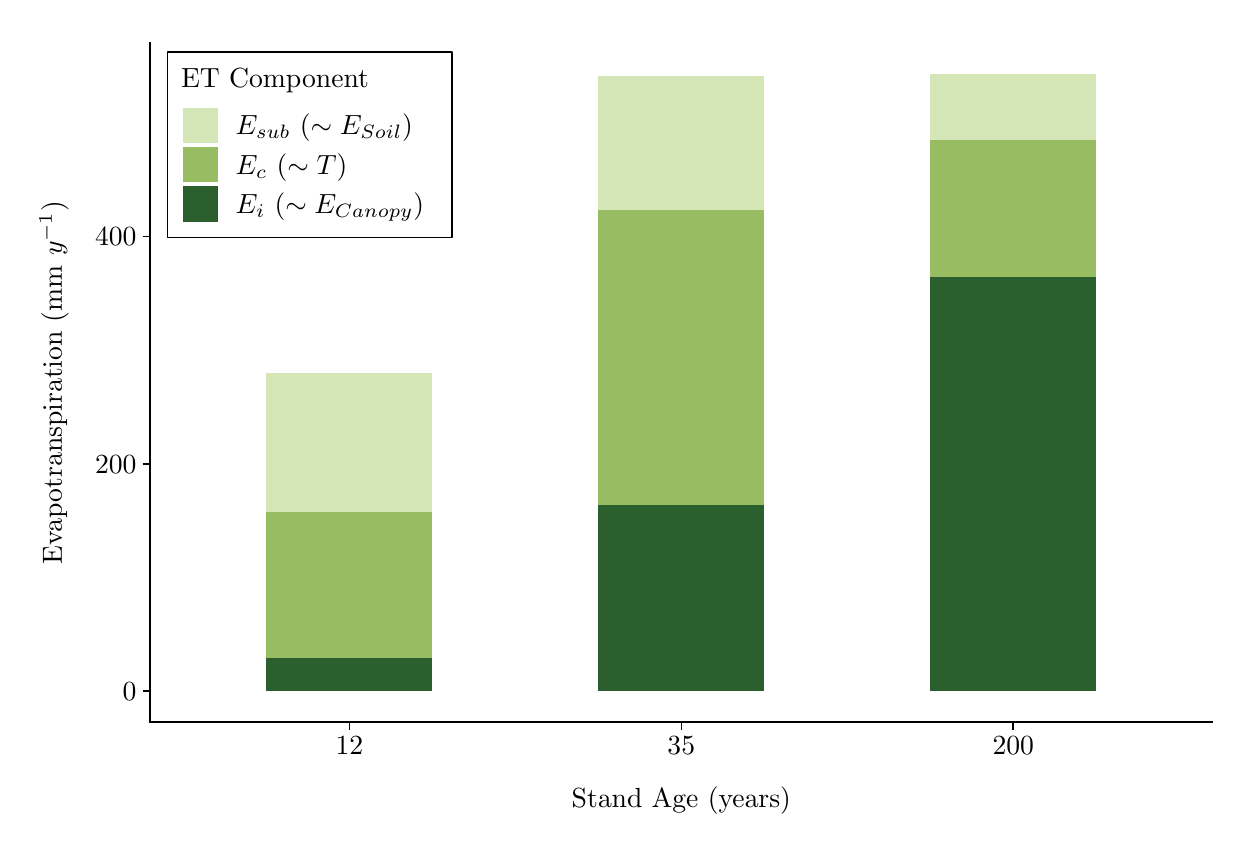
\begin{tikzpicture}[x=1pt,y=1pt]
\definecolor{fillColor}{RGB}{255,255,255}
\path[use as bounding box,fill=fillColor,fill opacity=0.00] (0,0) rectangle (433.62,289.08);
\begin{scope}
\path[clip] (  0.00,  0.00) rectangle (433.62,289.08);
\definecolor{drawColor}{RGB}{255,255,255}
\definecolor{fillColor}{RGB}{255,255,255}

\path[draw=drawColor,line width= 0.6pt,line join=round,line cap=round,fill=fillColor] (  0.00,  0.00) rectangle (433.62,289.08);
\end{scope}
\begin{scope}
\path[clip] ( 44.28, 38.11) rectangle (428.12,283.58);
\definecolor{fillColor}{RGB}{255,255,255}

\path[fill=fillColor] ( 44.28, 38.11) rectangle (428.12,283.58);
\definecolor{fillColor}{RGB}{212,230,181}

\path[fill=fillColor] ( 86.26,114.20) rectangle (146.24,164.34);
\definecolor{fillColor}{RGB}{151,188,98}

\path[fill=fillColor] ( 86.26, 61.19) rectangle (146.24,114.20);
\definecolor{fillColor}{RGB}{44,95,46}

\path[fill=fillColor] ( 86.26, 49.27) rectangle (146.24, 61.19);
\definecolor{fillColor}{RGB}{212,230,181}

\path[fill=fillColor] (206.21,223.11) rectangle (266.19,271.60);
\definecolor{fillColor}{RGB}{151,188,98}

\path[fill=fillColor] (206.21,116.67) rectangle (266.19,223.11);
\definecolor{fillColor}{RGB}{44,95,46}

\path[fill=fillColor] (206.21, 49.27) rectangle (266.19,116.67);
\definecolor{fillColor}{RGB}{212,230,181}

\path[fill=fillColor] (326.16,248.59) rectangle (386.14,272.42);
\definecolor{fillColor}{RGB}{151,188,98}

\path[fill=fillColor] (326.16,198.86) rectangle (386.14,248.59);
\definecolor{fillColor}{RGB}{44,95,46}

\path[fill=fillColor] (326.16, 49.27) rectangle (386.14,198.86);
\end{scope}
\begin{scope}
\path[clip] (  0.00,  0.00) rectangle (433.62,289.08);
\definecolor{drawColor}{RGB}{0,0,0}

\path[draw=drawColor,line width= 0.6pt,line join=round,line cap=rect] ( 44.28, 38.11) --
	( 44.28,283.58);
\end{scope}
\begin{scope}
\path[clip] (  0.00,  0.00) rectangle (433.62,289.08);
\definecolor{drawColor}{RGB}{0,0,0}

\node[text=drawColor,anchor=base east,inner sep=0pt, outer sep=0pt, scale=  1.00] at ( 39.33, 45.83) {0};

\node[text=drawColor,anchor=base east,inner sep=0pt, outer sep=0pt, scale=  1.00] at ( 39.33,128.02) {200};

\node[text=drawColor,anchor=base east,inner sep=0pt, outer sep=0pt, scale=  1.00] at ( 39.33,210.21) {400};
\end{scope}
\begin{scope}
\path[clip] (  0.00,  0.00) rectangle (433.62,289.08);
\definecolor{drawColor}{RGB}{0,0,0}

\path[draw=drawColor,line width= 0.6pt,line join=round] ( 41.53, 49.27) --
	( 44.28, 49.27);

\path[draw=drawColor,line width= 0.6pt,line join=round] ( 41.53,131.46) --
	( 44.28,131.46);

\path[draw=drawColor,line width= 0.6pt,line join=round] ( 41.53,213.65) --
	( 44.28,213.65);
\end{scope}
\begin{scope}
\path[clip] (  0.00,  0.00) rectangle (433.62,289.08);
\definecolor{drawColor}{RGB}{0,0,0}

\path[draw=drawColor,line width= 0.6pt,line join=round,line cap=rect] ( 44.28, 38.11) --
	(428.12, 38.11);
\end{scope}
\begin{scope}
\path[clip] (  0.00,  0.00) rectangle (433.62,289.08);
\definecolor{drawColor}{RGB}{0,0,0}

\path[draw=drawColor,line width= 0.6pt,line join=round] (116.25, 35.36) --
	(116.25, 38.11);

\path[draw=drawColor,line width= 0.6pt,line join=round] (236.20, 35.36) --
	(236.20, 38.11);

\path[draw=drawColor,line width= 0.6pt,line join=round] (356.15, 35.36) --
	(356.15, 38.11);
\end{scope}
\begin{scope}
\path[clip] (  0.00,  0.00) rectangle (433.62,289.08);
\definecolor{drawColor}{RGB}{0,0,0}

\node[text=drawColor,anchor=base,inner sep=0pt, outer sep=0pt, scale=  1.00] at (116.25, 26.28) {12};

\node[text=drawColor,anchor=base,inner sep=0pt, outer sep=0pt, scale=  1.00] at (236.20, 26.28) {35};

\node[text=drawColor,anchor=base,inner sep=0pt, outer sep=0pt, scale=  1.00] at (356.15, 26.28) {200};
\end{scope}
\begin{scope}
\path[clip] (  0.00,  0.00) rectangle (433.62,289.08);
\definecolor{drawColor}{RGB}{0,0,0}

\node[text=drawColor,anchor=base,inner sep=0pt, outer sep=0pt, scale=  1.00] at (236.20,  7.44) {Stand Age (years)};
\end{scope}
\begin{scope}
\path[clip] (  0.00,  0.00) rectangle (433.62,289.08);
\definecolor{drawColor}{RGB}{0,0,0}

\node[text=drawColor,rotate= 90.00,anchor=base,inner sep=0pt, outer sep=0pt, scale=  1.00] at ( 12.39,160.85) {Evapotranspiration (mm $y^{-1}$)};
\end{scope}
\begin{scope}
\path[clip] (  0.00,  0.00) rectangle (433.62,289.08);
\definecolor{drawColor}{RGB}{0,0,0}
\definecolor{fillColor}{RGB}{255,255,255}

\path[draw=drawColor,line width= 0.5pt,line join=round,line cap=round,fill=fillColor] ( 50.42,213.25) rectangle (153.29,280.27);
\end{scope}
\begin{scope}
\path[clip] (  0.00,  0.00) rectangle (433.62,289.08);
\definecolor{drawColor}{RGB}{0,0,0}

\node[text=drawColor,anchor=base west,inner sep=0pt, outer sep=0pt, scale=  1.00] at ( 55.42,267.41) {ET Component};
\end{scope}
\begin{scope}
\path[clip] (  0.00,  0.00) rectangle (433.62,289.08);
\definecolor{fillColor}{RGB}{255,255,255}

\path[fill=fillColor] ( 55.42,246.71) rectangle ( 69.65,260.93);
\definecolor{fillColor}{RGB}{212,230,181}

\path[fill=fillColor] ( 56.13,247.42) rectangle ( 68.94,260.22);
\end{scope}
\begin{scope}
\path[clip] (  0.00,  0.00) rectangle (433.62,289.08);
\definecolor{fillColor}{RGB}{255,255,255}

\path[fill=fillColor] ( 55.42,232.48) rectangle ( 69.65,246.71);
\definecolor{fillColor}{RGB}{151,188,98}

\path[fill=fillColor] ( 56.13,233.19) rectangle ( 68.94,246.00);
\end{scope}
\begin{scope}
\path[clip] (  0.00,  0.00) rectangle (433.62,289.08);
\definecolor{fillColor}{RGB}{255,255,255}

\path[fill=fillColor] ( 55.42,218.25) rectangle ( 69.65,232.48);
\definecolor{fillColor}{RGB}{44,95,46}

\path[fill=fillColor] ( 56.13,218.97) rectangle ( 68.94,231.77);
\end{scope}
\begin{scope}
\path[clip] (  0.00,  0.00) rectangle (433.62,289.08);
\definecolor{drawColor}{RGB}{0,0,0}

\node[text=drawColor,anchor=base west,inner sep=0pt, outer sep=0pt, scale=  1.00] at ( 75.15,250.38) {$E_{sub}$ ($\sim E_{Soil})$};
\end{scope}
\begin{scope}
\path[clip] (  0.00,  0.00) rectangle (433.62,289.08);
\definecolor{drawColor}{RGB}{0,0,0}

\node[text=drawColor,anchor=base west,inner sep=0pt, outer sep=0pt, scale=  1.00] at ( 75.15,236.15) {$E_c$ ($\sim T)$};
\end{scope}
\begin{scope}
\path[clip] (  0.00,  0.00) rectangle (433.62,289.08);
\definecolor{drawColor}{RGB}{0,0,0}

\node[text=drawColor,anchor=base west,inner sep=0pt, outer sep=0pt, scale=  1.00] at ( 75.15,221.92) {$E_i$ ($\sim E_{Canopy})$};
\end{scope}
\end{tikzpicture}
